\documentclass{article}
\usepackage{amsmath}
\usepackage{graphicx}
\usepackage{booktabs}
\usepackage{ctex}
\usepackage{hyperref}

\title{三维分形生成：基于 VQ-VAE 的由粗到细八叉树生成}
\author{余东格}
\date{2026 年 7 月}

\begin{document}

\maketitle

\section{研究背景与问题}
三维形状的生成如果在稠密体素上直接建模，会在大量空白区域浪费算力。八叉树把形状表示为
由粗到细的层级结构：先在低分辨率判断大致占据区域，再逐层只在被占据的节点上细分，从而
把计算集中在形状表面附近。OctGPT 沿这一思路，用一个自回归 Transformer 逐 token 生成
八叉树，并配合一个冻结的 VQ-VAE 把叶子层的离散 token 解码为连续 SDF，质量很高，但代价
是迭代式解码：每个样本需要约 576 次前向（各层 MaskGIT 迭代步数 $[64,128,128,256]$），
单样本推理约 43 秒。

本工作的核心研究问题是：\emph{一个单次前向（约 4 次 forward）的由粗到细生成器，能否
逼近 OctGPT 这类迭代自回归模型的形状质量}，从而以远低的推理成本换取可比的形状。我们
复用 OctGPT 完全相同的冻结 VQ-VAE 作为叶子解码器，只把生成器换成由粗到细、少步前向的
结构，这样质量差异可以干净地归因到生成器本身，而非解码器。

\section{方法}
生成器只负责预测八叉树结构与叶子层的 VQ token，解码交给冻结的 VQ-VAE。整体流程为：
逐层预测 split $\rightarrow$ 展开到 \texttt{depth\_stop}=6 $\rightarrow$ 叶子层预测
VQ token $\rightarrow$ 冻结 VQ-VAE 解码为 SDF $\rightarrow$ marching cubes 得到网格。
主要组成部分：

\begin{itemize}
    \item \textbf{由粗到细的 split 预测：} 从 \texttt{full\_depth}=3 起，用 OctFormer
    逐层预测每个节点是否分裂，展开至 \texttt{depth\_stop}=6，再由 zero split 扩到
    \texttt{depth}=8。父节点通过局部 cross-attention 展开为 8 个子节点。
    \item \textbf{叶子层 VQ token 与冻结解码器：} 叶子层预测离散 VQ token，由冻结
    VQ-VAE 解码为连续 SDF，使叶子表示具备比纯占据更强的表面细节。
    \item \textbf{条件化：} 原始无条件模型生成严重趋同（所有样本几乎相同）。为此引入
    类别嵌入与 VAE 隐变量 $z$（$z$ 由真值形状编码得到，生成时从 $\mathcal{N}(0,I)$
    采样），并在\emph{每一层}注入条件。所有条件相关权重 zero-init，使加入条件后与
    warm-start 起点严格等价。
    \item \textbf{sibling attention：} 父节点展开为 8 个子节点时，原本的
    cross-attention 上下文长度为 1，退化为逐节点 MLP，8 个兄弟节点之间不通信。加入
    sibling self-attention 让同一父节点的 8 个八分体子节点互相 attend（真正的 $K=8$
    注意力），得到更好的子节点特征，进而改善 split 预测。
    \item \textbf{split 监督：} 节点是否分裂存在严重类别不平衡（split=1 很稀疏），
    采用 Focal Loss 监督。训练用 teacher forcing，沿真值八叉树逐层展开并监督每个
    节点的 split 与叶子 token。
\end{itemize}

\section{单飞机过拟合验证}
首先在单个飞机样本上过拟合，确认从 split 预测、VQ token 预测到 VQ-VAE 解码与 OBJ
导出的完整 pipeline 是可学习的。把消融中表现较好的结构性改动（sibling attention、
粗层容量、全局 buffer）微调到单飞机上，split accuracy 收敛到 0.998（末层），
VQ accuracy 约 0.847。结构（split）几乎完美，说明八叉树拓扑被准确学到、整条实现有效。

值得注意的是，早期导出的网格表面满布小孔。为定位这一现象的来源，我们做了一个
\emph{oracle 对照}：把真值形状的叶子 token（经冻结 VQ-VAE 编码量化得到）直接送回
同一个冻结 VQ-VAE 解码，得到``解码器上限''网格，再与我们生成器的输出并排比较
（图~\ref{fig:overfit}）。二者几乎一致：oracle 与本方法生成的平均二面角分别为
$14.0^\circ$ 与 $13.2^\circ$，$>60^\circ$ 的棱占比都是 $2.6\%$。这说明小孔\emph{并非}
来自我们生成器的 split 或 token 误差。进一步排查发现真正的来源是 marching cubes 的
等值面取值：默认 $\ell=0.002$ 恰好落在冻结解码器输出 SDF 的零点噪声带内，任何表面附近
的微小符号抖动都会被抠成孔洞；把等值面提高到 $\ell=0.01$（对 depth-8、体素约
$2/256$ 的尺度而言仍是极薄的偏移）后，oracle 与生成结果的小孔同时消失，且该修复
\emph{无需任何重训练}。图~\ref{fig:overfit}即为 $\ell=0.01$ 下的对照：上排 oracle、
下排本方法，二者形状与表面质量几乎一致，机身、后掠翼、尾翼清晰可辨。换言之，在这个
过拟合样本上，约 4 次前向的生成器已经达到了解码器自身的重建上限。

\begin{figure}[htbp]
    \centering
    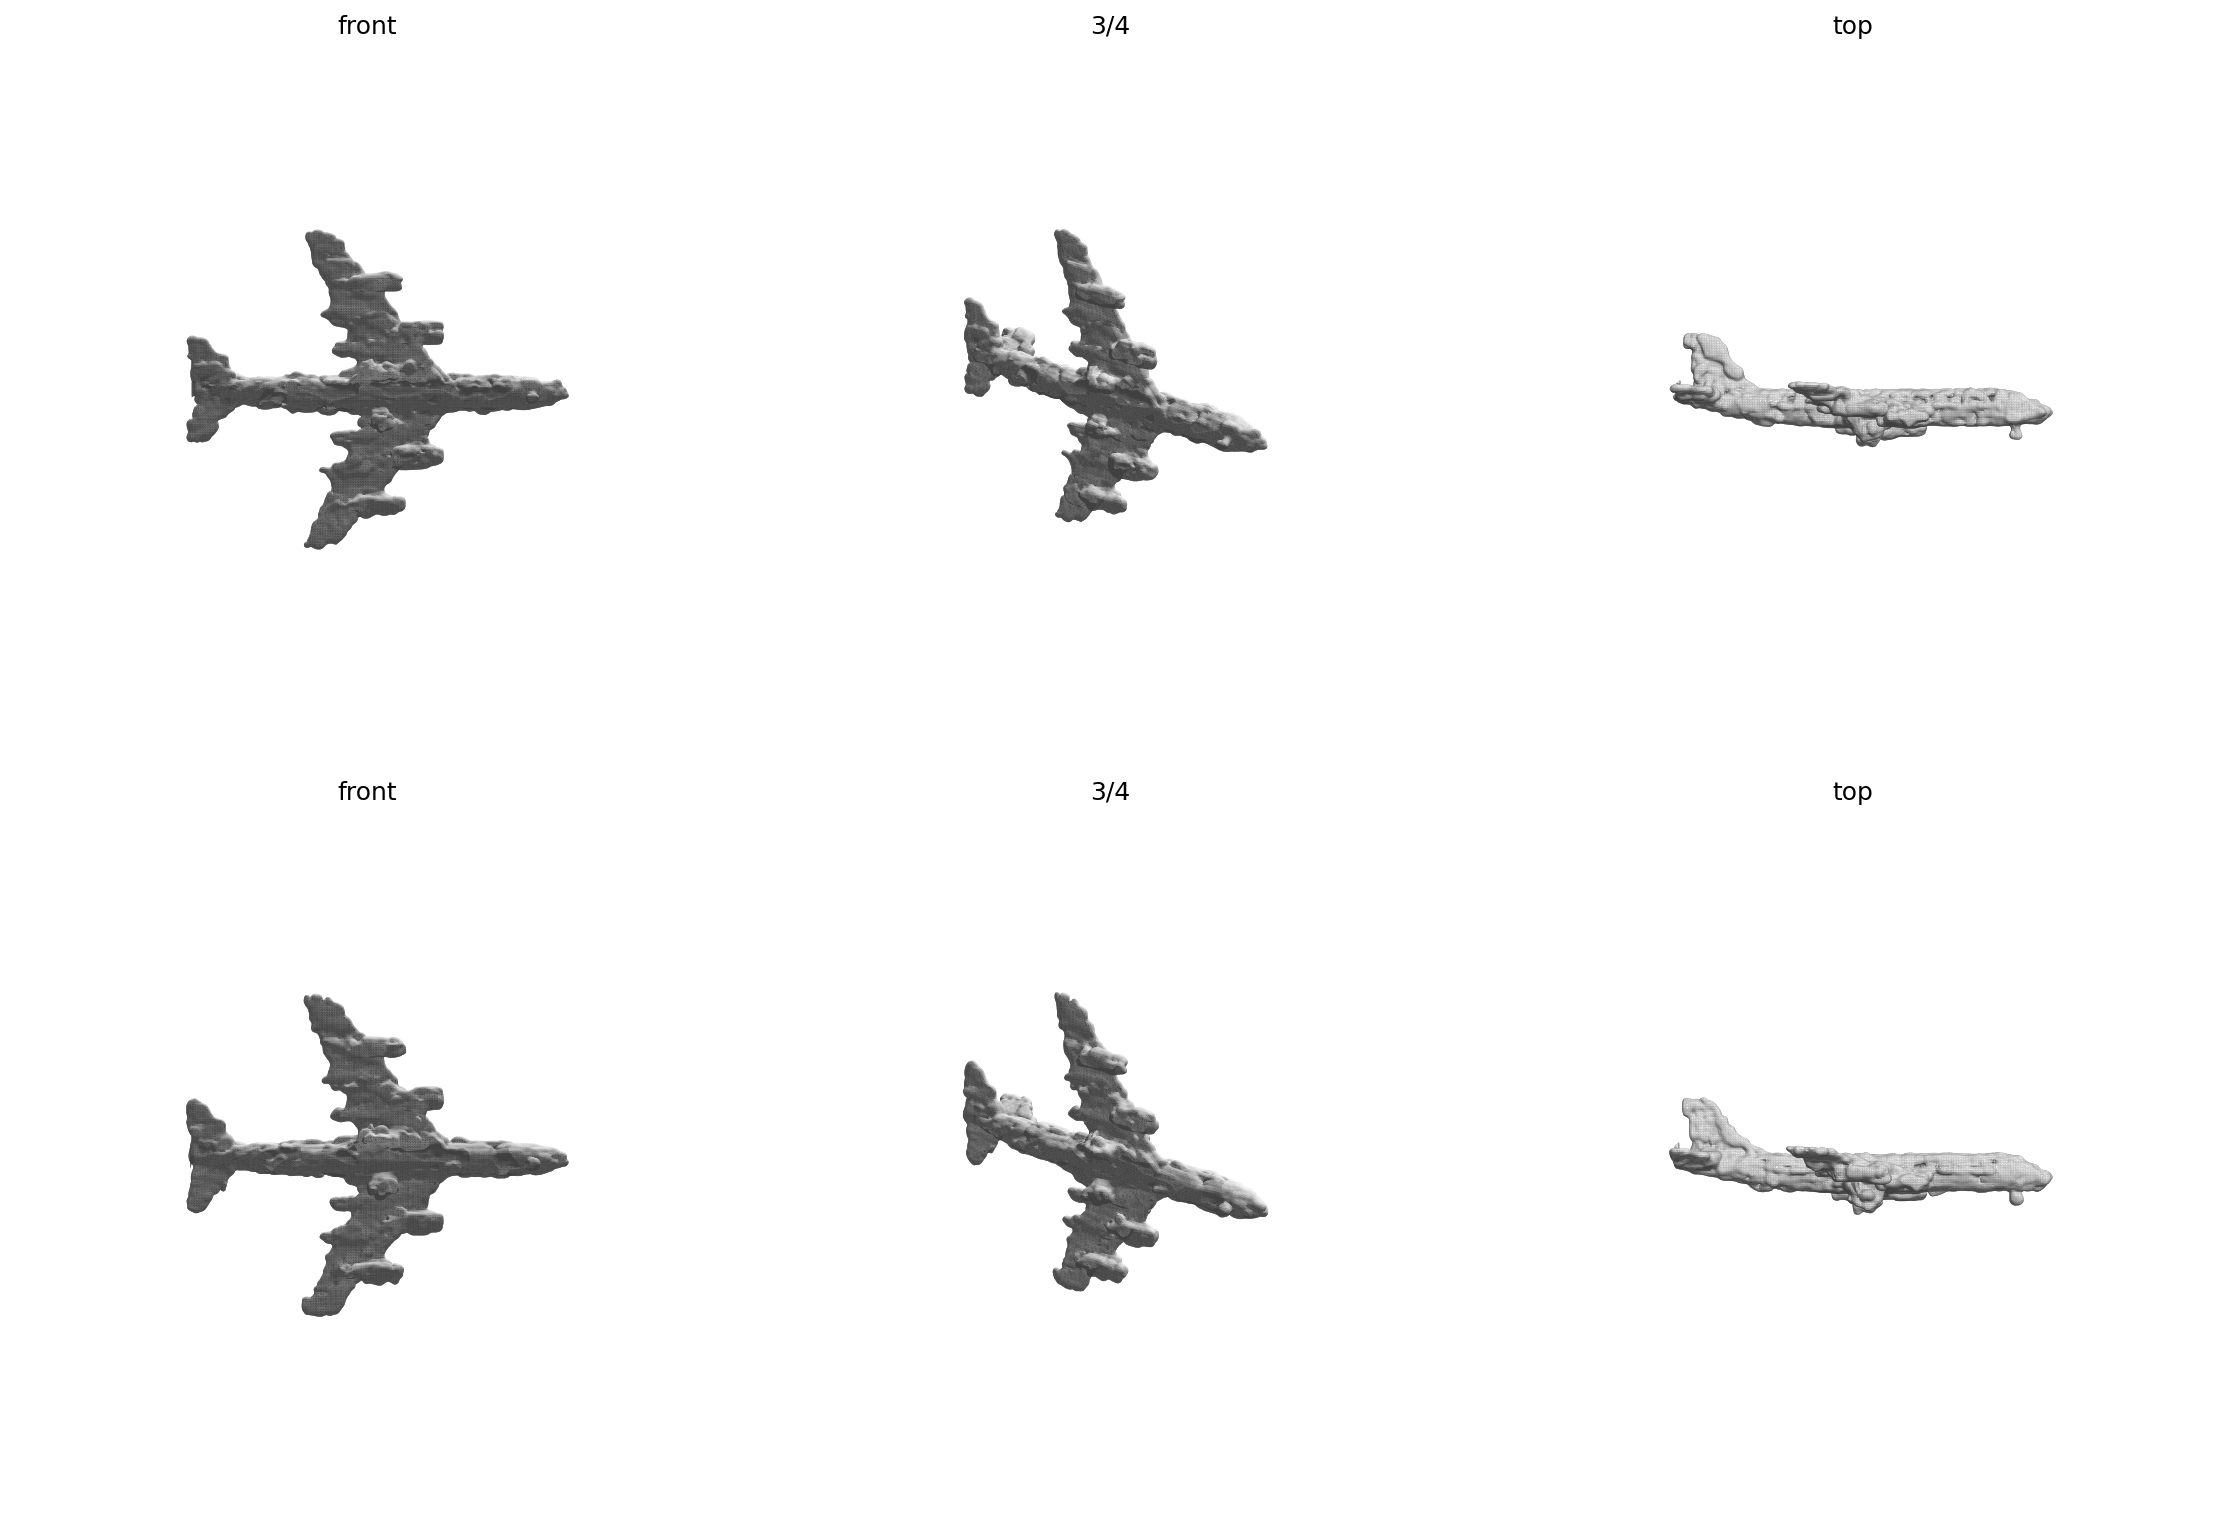
\includegraphics[width=0.92\linewidth]{airplane_overfit.png}
    \caption{单飞机过拟合的 oracle 对照（正视 / 3/4 视角 / 顶视，marching cubes
    等值面 $\ell=0.01$）。上排为真值 token 经同一冻结 VQ-VAE 解码得到的``解码器
    上限''，下排为本方法约 4 次前向的自由生成结果。二者形状与表面质量几乎一致，
    表明生成器已达到解码器自身在 depth-6 的重建上限。}
    \label{fig:overfit}
\end{figure}

\section{多类别消融（im-5）}
在多类别 im-5 数据集（airplane / car / chair / rifle / table 五类）上，我们做了
条件化、latent、模型扩容与迭代式 refinement 的消融。主要结果如表~\ref{tab:ablation}，
指标为最后一层 split accuracy 与 VQ accuracy；参照是无条件 baseline。

\begin{table}[htbp]
    \centering
    \begin{tabular}{llccc}
        \toprule
        实验 & 主要改动 & split acc & 末层 split acc & VQ acc \\
        \midrule
        --  & 无条件 baseline（生成趋同） & $\sim$0.79 & --    & --    \\
        C2  & 类别条件每层注入            & 0.812      & 0.756 & 0.652 \\
        V1  & C2 + latent $z$             & 0.836      & 0.780 & 0.647 \\
        Q2  & 768 维大模型                & 0.840      & 0.788 & 0.646 \\
        Q3  & Q2 + split MaskGIT          & 0.836      & 0.776 & 0.644 \\
        Q4  & Q2 + sibling attention      & 0.841--0.845 & 0.795--0.800 & 0.645--0.647 \\
        S1  & V1 + leaf VQ MaskGIT        & 0.840      & 0.791 & 0.639 \\
        \bottomrule
    \end{tabular}
    \caption{VQ-VAE 分形生成路线在 im-5 多类别数据上的主要消融结果。}
    \label{tab:ablation}
\end{table}

如实来看：

\begin{itemize}
    \item \textbf{条件化是关键。} 无条件模型退化为预测边缘分布、样本趋同，split acc
    停在约 0.79。加入类别条件与 latent $z$（C2、V1）明显缓解趋同，不同类别可生成不同
    形状，split acc 提升到 0.84 附近。
    \item \textbf{扩容与 sibling 只有小幅增益。} 768 维大模型（Q2）与 sibling
    attention（Q4）带来小幅结构提升，Q4 是当前结构指标最好的版本（末层 split acc
    约 0.80），但增益已很有限。
    \item \textbf{迭代式 refinement 是负结果。} Q3 的 split-MaskGIT 没有达到预期，
    迭代反而使结构变稀疏、碎片增多；它与特征级联式的单次前向架构不匹配。leaf VQ
    MaskGIT（S1）对 nearest-CD 有一定趋势，但 S1 用的是 384 维配置，与 768 维的 Q4
    不是严格同容量对照，不能直接比较。
\end{itemize}

\section{空洞来源诊断与结构改进}
\label{sec:diag}
多类别生成的网格长期存在``缺块/空洞、散点''的问题。表~\ref{tab:ablation}中的
split accuracy 无法解释它：该指标被大量``不分裂''的负样本主导，掩盖了真正致命的错误
类型。为此我们为每一层单独统计 split=1 类的查全率（recall）与查准率（precision），
并构建了一个逐层按八叉树 key 对齐生成结构与真值结构的诊断工具，得到两个关键事实：

\begin{itemize}
    \item \textbf{漏分裂的代价高度不对称。} depth $d$ 上漏掉一个本应分裂的节点，会
    砍掉整棵子树（至多 $8^{\,6-d}$ 个叶子），造成整块几何缺失；反之多分裂只是表面
    变密。因此 recall 远比 accuracy 重要。
    \item \textbf{瓶颈在最粗层而非最细层。} 以结构最好的 Q4 为例，teacher-forcing
    下按生成阈值判决，depth-3（最粗层）的漏分裂率高达 21.4\%（每个漏判平均丢约 57 个
    叶子），而 depth-5 仅 5.7\%；自由生成时粗层错误逐层级联，depth-6 叶子缺失率达
    29.3\%，结构 IoU 仅 0.33。此前报告聚焦``末层 accuracy 约 0.80''是被指标定义
    误导的结论。
\end{itemize}

诊断同时给出了两个\emph{免训练}的生成端修复：叶子 token 改用 argmax
（temperature=0，消除 VQ 采样噪声在 0.65 左右的 token 准确率下渲染成的``雪花''）、
marching cubes 等值面 $\ell=0.01$（第 3 节）。二者叠加使 chair/car 等类别从噪声云
变为轮廓清晰的实体。

针对粗层瓶颈，我们在 Q4 基础上引入两个训练侧改动（记为 R2，warm-start 自 Q4）：
\textbf{(1) 粗层加权 split loss}，按子树代价给各层 loss 乘以 $[4,2,1]$ 权重；
\textbf{(2) 空间池化 latent}：原 $z$ 是叶子 VQ code 的全局平均，不含空间布局信息，
诊断显示模型完全忽略它（用真值后验 $z$ 与先验采样 $z$ 生成的结构完全相同）；改为按
$8^3=512$ 个 depth-3 空间格分别池化后再编码，使 $z$ 携带粗层布局。%
% TODO(ep30): 用 epoch-30 最终数字刷新本段
在 im-5 上训练 20 epoch 后：depth-3 recall 从 0.786 升至 0.950，自由生成叶子缺失率
从 29.3\% 降至约 5\%，结构 IoU 0.33 $\to$ 0.44，VQ accuracy 0.645 $\to$ 0.681，
且后验/先验 $z$ 的生成结构不再相同（latent 开始生效）。但代价是细层查准率降至约
0.75：模型整体向``宁多勿漏''偏移，多余的分裂把机翼间隙等凹陷填成实心，airplane/car
的轮廓反而变差，而 chair/rifle/table 改善。这揭示了单次前向框架下 recall 与轮廓
质量之间的张力，我们在第~6 节进一步讨论其根源。

\section{速度对比}
主要卖点是推理成本。生成器前向次数约 4 次（由粗到细逐层各一次）对比 OctGPT 的约
576 次迭代解码，且两者共用同一冻结 VQ-VAE。实测见表~\ref{tab:speed}。

\begin{table}[htbp]
    \centering
    \begin{tabular}{lccc}
        \toprule
        方法 & 前向次数/样本 & 生成器耗时 & 端到端（含 marching cubes） \\
        \midrule
        OctGPT（官方权重，实测） & $\sim$576 & $\sim$77 s  & $\sim$81 s \\
        本方法（单次前向）       & $\sim$4   & $\sim$0.23 s & $\sim$3.8 s \\
        \bottomrule
    \end{tabular}
    \caption{推理速度对比（同一台 A100、同一冻结 VQ-VAE、res=256）。OctGPT 为官方
    发布的 airplane 权重实测（每样本约 81 s）；本方法生成器约 4 次前向、0.23 s。
    生成器部分约 300 倍加速，端到端约 21 倍；端到端瓶颈是两者共享的 marching cubes
    （res=256 约 3.5 s）。}
    \label{tab:speed}
\end{table}

\begin{figure}[htbp]
    \centering
    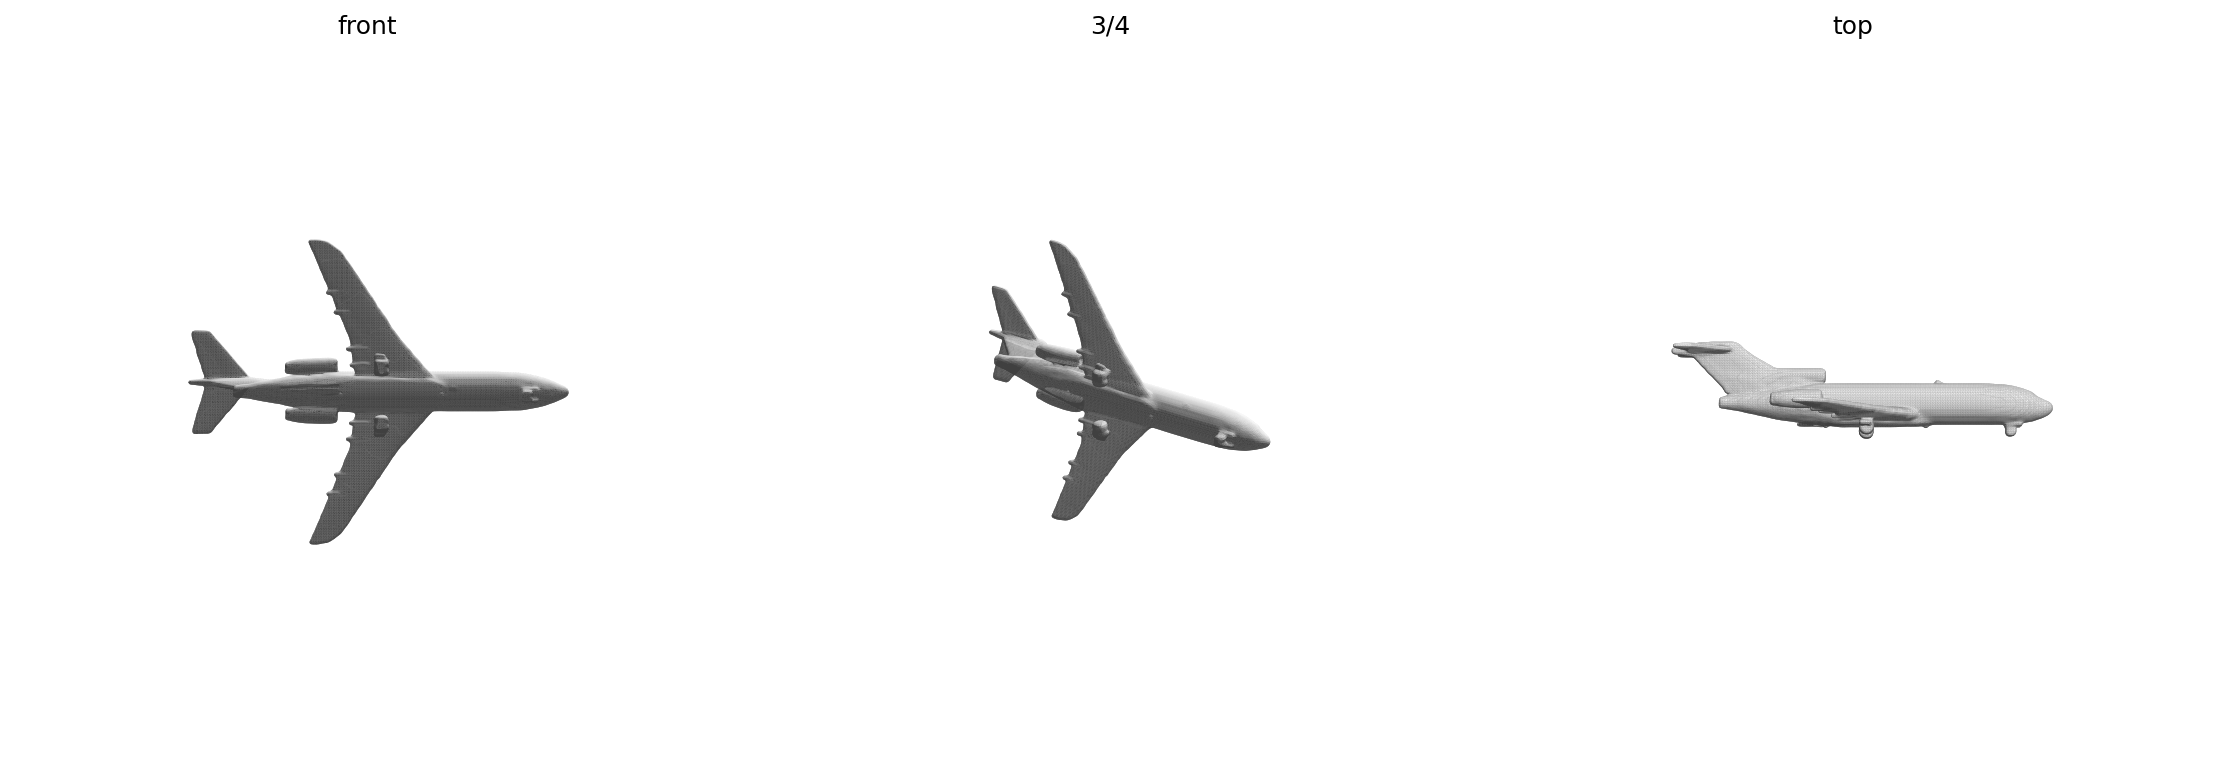
\includegraphics[width=0.92\linewidth]{octgpt_airplane_baseline.png}
    \caption{OctGPT 官方 airplane 权重配同一冻结 VQ-VAE 的生成样本（实测约 81 s
    /样本）。它验证了两件事：解码器本身有能力输出光滑表面（我们多类别结果的表面
    粗糙主要来自 token 预测质量而非解码器），以及迭代式生成在轮廓上仍显著优于
    单次前向，这正是表~\ref{tab:speed}中速度优势所换取的代价。}
    \label{fig:octgpt}
\end{figure}

生成器部分约 300 倍加速；端到端约 21 倍，其瓶颈是两种方法共享的 marching cubes
（res=256 约 3.5 秒，res=512 约 20 秒），并非生成器本身。

\section{结论与不足}
本工作搭通了 ``由粗到细 split 预测 + 叶子 VQ token + 冻结 VQ-VAE 解码 + marching
cubes'' 的完整训练与生成流程，在单飞机上验证了 pipeline 可完整拟合，并在 im-5 多类别
上通过条件化修复了生成趋同问题，同时在推理速度上相对 OctGPT 有明显优势。主要不足：

\begin{itemize}
    \item \textbf{根本限制：独立边缘判决的模式平均。} 单次前向对每个节点按
    \emph{独立的边缘概率}判决是否分裂。当类内存在多种布局模式（不同机翼位置、不同
    桌腿结构）时，各节点的边缘概率被拉向多模式的平均，生成结果趋向``类别平均形状''
    （飞机的实心三角翼团块即由此而来）。空间池化 latent 缓解但不足以完全消除；
    OctGPT 的 576 步迭代每步都以已确定的部分结构为条件、逐步承诺到单一模式，这正是
    质量差距的本质来源。
    \item \textbf{recall 与轮廓质量的张力。} 第~\ref{sec:diag} 节的 R2 实验显示：
    把粗层漏分裂率从 21\% 压到 5\% 的同时，细层查准率跌至约 0.75，过度分裂把凹陷
    填成实心。在``独立判决''框架内，向 recall 倾斜与保持轮廓锐利难以两全。
    \item \textbf{表面细节受限于 token 质量。} OctGPT 官方权重配同一解码器可输出
    光滑表面（图~\ref{fig:octgpt}），说明解码器不是上限；我们多类别 VQ accuracy
    仅约 0.68，token 误差在表面上渲染为颗粒感，argmax 采样与 $\ell=0.01$ 只能部分
    掩盖。
\end{itemize}

基于以上分析，最有希望的后续方向是\emph{仅在最粗层引入少步迭代}：depth-3 只有至多
512 个节点，做 4--8 步 MaskGIT 式 refinement 仅增加约 8 次前向（总前向仍
$\sim$12 次，保持约 50 倍生成器加速），却把``模式承诺''引入了错误代价最高的一层。
它与已失败的全层 split-MaskGIT（Q3）的区别在于只作用于粗层且训练/生成策略匹配。
此外还应补齐 MMD-CD / COV / 1-NNA 量化指标，在``速度--质量''曲线上系统对比本方法
与 OctGPT。

\end{document}
